\chapter{Introduction to Security Testing}
	\clearpage
	\section{The OWASP Testing Guide}
		{\bf OWASP:} The Open Web Application Security Project

		The OWASP Testing Project has been in development for many years. With this project, 
		we wanted to help people understand the what, why, when, where, and how of testing their 
		web applications, and not just provide a simple checklist or prescription of issues 
		that should be addressed. The outcome of this project is a complete Testing Framework, 
		from which others can build their own testing programs or qualify other people’s 
		processes. The Testing Guide describes in details both the general Testing Framework and 
		the techniques required to implement the framework in practice.

		\section{What, Why, When?}

		{\bf What is Testing?} \\
		What do we mean by testing? During the development life cycle of a web application, 
		many things need to be tested. The Merriam-Webster Dictionary describes testing as:
			\begin{itemize}
				\item To put to test or proof.
				\item To undergo a test.
				\item To be assigned a standing or evaluation based on tests.
			\end{itemize}
		Many outsiders regard security testing as a black art. This document’s aim is to
		change that perception and to make it easier for people without in-depth security 
		knowledge to make a difference.

		{\bf Why Testing?} \\
		This document is designed to help organizations understand what comprises a testing 
		program, and to help them identify the steps that they need to undertake to build 
		and operate that testing program on their web applications. 
		It is intended to give a broad view of the elements required to make a comprehensive 
		web application security program. 
		This guide can be used as a reference and as a methodology to help determine the gap 
		between your existing practices and industry best practices. 
		This guide allows organizations to compare themselves against industry peers, understand 
		the magnitude of resources required to test and maintain their software, or prepare for 
		an audit. 
		The technical details about how to test an application, as part of a penetration test or code review, will be covered in later chapters. 

		\clearpage
		{\bf When to Test?} \\ 
		Most people today don’t test the software until it has already been created and is in 
		the deployment phase of its life cycle (i.e., code has been created and instantiated 
		into a working web application). 
		This is generally a very ineffective and cost-prohibitive practice. One of the best 
		methods to prevent security bugs from appearing in production applications is to 
		improve the Software Development Life Cycle (SDLC) by including security in each of 
		its phases. 

		An SDLC is a structure imposed on the development of software artifacts. If an SDLC 
		is not currently being used in your environment, it is time to pick one! 
		The following figure shows a generic SDLC model: 

		\begin{figure} [H]
			\centering
			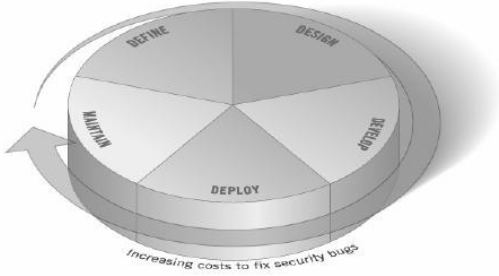
\includegraphics[scale=0.5]{pics/SDCL.png}
		\end{figure}


		{\bf What to Test?} \\
		It can be helpful to think of software development as a combination of people, process, 
		and technology. If these are the factors that "create" software, then it is logical 
		that these are the factors that must be tested. Today most people generally
		test the technology or the software itself. An effective testing program should 
		have components that test \\
		{\bf People} – to ensure that there is adequate education and
		awareness; \\ 
		{\bf Process} – to ensure that there are adequate policies and standards and 
		that people know how to follow these policies; \\ 
		{\bf Technology} – to ensure that the process has been effective in its implementation. 

		\clearpage
		\section{Principles of Testing}

			{\bf There is no silver bullet: } While it is tempting to think that a security 
			scanner or application firewall will either provide a multitude of defenses or
			identify a multitude of problems, in reality there are no silver bullets to the 
			problem of insecure software.

			{\bf Think strategically, not tactically: } The patch-and-penetrate model involves
			fixing a reported bug, but without proper investigation of the root cause. 
			This model is usually associated with the window of vulnerability:

				\begin{figure}[H]
					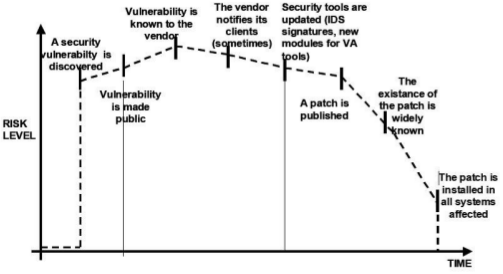
\includegraphics[scale=0.7]{pics/windowOfExposure.png}
				\end{figure}


			To prevent reoccurring security problems within an application, it is essential 
			to build security into the Software Development Life Cycle (SDLC) by developing
			standards, policies, and guidelines that fit and work within the development
			methodology. Threat modeling and other techniques should be used to help assign
			appropriate resources to those parts of a system that are most at risk.


			{\bf Test early and test often: } When a bug is detected early within the SDLC, 
			it can be addressed more quickly and at a lower cost. A security bug is no
			different from a functional or performance-based bug in this regard.


			{\bf Understand the scope of security:} It is important to know how much security 
			a given project will require. The information and assets that are to be protected
			should be given a classification that states how they are to be handled (e.g., Confidential, Secret, Top Secret). Security testing cost money! You have to
			prioritize what's important for your system. 

			\clearpage
			{\bf Develop the right mindset: } Successfully testing an application for security
			vulnerabilities requires thinking "outside of the box." Normal use cases will
			test the normal behavior of the application when a user is using it in the manner 
			that you expect. Good security testing requires going beyond what is expected and
			thinking like an attacker who is trying to break the application. This is one of 
			the reasons why automated tools are actually bad at automatically testing for
			vulnerabilities.

			{\bf Understand the subject: } One of the first major initiatives in any good 
			security program should be to require accurate documentation of the application. 
			The architecture, data-flow diagrams, use cases, and more should be written in 
			formal documents and made available for review. 

			{\bf Use the right tools: } While we have already stated that there is no silver 
			bullet tool. There is a range of open source and commercial tools that can 
			automate many routine security tasks. These tools can simplify and speed up the 
			security process. It is important to understand exactly what these tools can 
			and cannot do.

			{\bf The devil is in the details: } It is critical not to perform a superficial
			security review of an application and consider it complete. Care should be taken 
			to verify that every possible section of application logic has been tested, and 
			that every use case scenario was explored for possible vulnerabilities.

			{\bf Use source code when available: } While black box penetration test results 
			can be impressive and useful to demonstrate how vulnerabilities are exposed in
			production, they are not the most effective way to secure an application. 
			If the source code for the application is available, it should be given to the 
			security staff to assist them while performing their review. 
			It is possible to discover vulnerabilities within the application source that 
			would be missed during a black box engagement.

			{\bf Develop metrices: } An important part of a good security program is the 
			ability to determine if things are getting better. It is important to track
			the results of testing engagements, and develop metrics that will reveal the
			application security trends within the organization. 

			{\bf Document the test results: } To conclude the testing process, it is 
			important to produce a formal record of what testing actions were taken, 
			by whom, when they ware performed, and details of the test findings.


	\clearpage
	\section{Testing Techniques}

		This section presents a high-level overview of various testing techniques that 
		can be employed when building a testing program.

		\subsection{Manual Inspection and Reviews}
			Manual inspections are human-driven reviews that typically test the security
			implications of the people, policies, and processes, but can include inspection 
			of technology decisions such as architectural designs.
			By asking someone how something works and why it was implemented in a specific way, 
			it allows the tester to quickly determine if any security concerns are likely to 
			be evident. Manual inspections and reviews are one of the few ways to test
			the software development life-cycle process itself and to ensure that there is 
			an adequate policy or skill set in place. 
			As with many things in life, when conducting manual inspections and reviews we suggest you adopt a trust-but-verify model. 

			{\bf Advantages:}
			\begin{itemize}
				\item Requires no supporting technology
				\item Can be applied to a variety of situations
				\item Flexible
				\item Promotes teamwork
				\item Can be performed early in the SDLC
			\end{itemize}

			{\bf Disadvantages:}
			\begin{itemize}
				\item Can be time consuming
				\item Supporting material not always available
				\item Requires significant human thought and skill to be effective!
			\end{itemize}

		\clearpage
		\subsection{Threat Modeling}
			Threat modeling has become a popular technique to help system designers think 
			about the security threats that their systems/applications might face. 
			Therefore, threat modeling can be seen as risk assessment for applications. 
			In fact, it enables the designer to develop mitigation strategies for potential
			vulnerabilities and helps them focus their inevitably limited resources and 
			attention on the parts of the system that most require it.
			To develop a threat model, we recommend taking a simple approach.
			This approach involves:

			\begin{itemize}
				\item {\bf Defining and classifying the assets} – classify the assets into tangible and intangible assets and rank them according to business importance.
				\item {\bf Exploring potential vulnerabilities} - whether technical, operational, 
				or management.
				\item {\bf Decomposing the application} – how the application works, its assets,
				functionality, and connectivity.
				\item {\bf Exploring potential threats} – use threat scenarios and/or attack trees.
				\item {\bf Creating mitigation strategies} – develop mitigating controls for each of the threats deemed to be realistic.
			\end{itemize}

			{\bf Advantages:}
				\begin{itemize}
					\item Practical attacker's view of the system
					\item Flexible
					\item Early in the SDLC
				\end{itemize}

			{\bf Disadvantages:}
				\begin{itemize}
					\item Relatively new technique
					\item Good threat models don’t automatically mean good software
				\end{itemize}

		\clearpage
		\subsection{Source Code Review}
			Source code review is the process of manually checking a web application's source 
			code for security issues. Many serious security vulnerabilities cannot be detected 
			with any other form of analysis or testing. As the popular saying goes “if you
			want to know what’s really going on, go straight to the source." Almost all 
			security experts agree that there is no substitute for actually looking at the 
			code. All the information for identifying security problems is there in the code
			somewhere.

			{\bf Advantages:}
			\begin{itemize}
				\item Completeness and effectiveness
				\item Accuracy
				\item Fast (for competent reviewers)
			\end{itemize}
			{\bf Disadvantages:}
			\begin{itemize}
				\item Requires highly skilled security developers
				\item Can miss issues in compiled libraries
				\item Cannot detect run-time errors easily
				\item The source code actually deployed might differ from the one being analyzed
			\end{itemize}

		\clearpage	
		\subsection{Penetration Testing}

		Penetration testing has been a common technique used to test network security for 
		many years. It is also commonly known as black box testing or ethical hacking. 
		Penetration testing is essentially the “art” of testing a running application remotely,
		without knowing the inner workings of the application itself, to find security
		vulnerabilities. Typically, the penetration test team would have access to an 
		application as if they were users. The tester acts like an attacker and attempts 
		to find and exploit vulnerabilities. 
		Penetration testing tools have been developed that automate the
		process, but, again, with the nature of web applications their effectiveness is 
		usually poor. 

		Gary McGraw summed up penetration testing well when he said: \\
		{\bf “If you fail asummed penetration test you know you have a very bad problem indeed. 
		If you pass a penetration test you do not know that you don’t have a very bad problem”.}

		{\bf Advantages:}
		\begin{itemize}
			\item Can be fast (and therefore cheap)
			\item Requires a relatively lower skill-set than source code review
			\item Tests the code that is actually being exposed
		\end{itemize}

		{\bf Disadvantages:}
		\begin{itemize}
			\item Too late in the SDLC
			\item Front impact testing only!
		\end{itemize}

		\clearpage
		\subsection{Test Effort According to Test Technique}
			With so many techniques and so many approaches to testing the security of web
			applications, it can be difficult to understand which techniques to use and when 
			to use them. The fact remains that all techniques should probably be used to 
			ensure that all areas that need to be tested are tested. What is clear, however, 
			is that there is no single technique that effectively covers all security testing 
			that must be performed to ensure that all issues have been addressed. The following
			figure shows a typical proportional representation of test effort according to 
			test technique:

			\begin{figure}[H]
				\centering
				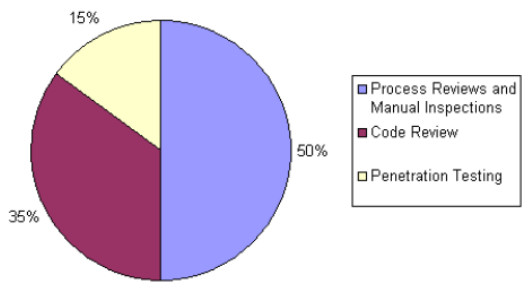
\includegraphics[scale=0.6]{pics/effort.png}
			\end{figure}

	\clearpage
	\section{Security Requirements}

		\subsection{Test Derivation}

		\subsection{Functional and Non-Functional Test Requirements}

		\subsection{Derivation Through Use and Misuse Cases}

		\subsection{Security Tests Integrated in Workflow}

		\subsection{Developers Security Tests}

		\subsection{Functional Testers' Security Tests}

		\subsection{Security Test Data Analysis and Reporting}


